%!TEX root = ../main.tex



\section{Εισαγωγή στους PID ελεγκτές}

\lettrine[findent=2pt]{\fbox{\textbf{Έ}}}{νας} αναλογικός-ολοκληρωτικός-παραγωγικός ελεγκτής (\emph{proportional-integral-derivative controller}) ή όπως είναι πιο γνωστός \emph{PID controller}, είναι ένας μηχανισμός ανάδρασης (\emph{feedback}) βρόχου ελέγχου (\emph{control loop}) που χρησιμοποιείται ευρέως σε βιομηχανικά συστήματα ελέγχου καθώς και σε μια ποικιλία άλλων εφαρμογών που απαιτούν συνεχή διαμορφωμένο έλεγχο. Η διαδικασία λειτουργίας είναι κοινή για όλους τους ελεγκτές αυτού του είδους. Ένας PID ελεγκτής υπολογίζει συνεχώς μια τιμή σφάλματος $e(t)$ ως διαφορά μεταξύ μιας επιθυμητής τιμής ρύθμισης (\emph{setpoint} ή \emph{SP}) και μεταξύ μιας μεταβλητής της διαδικασίας ύπο έλεγχο (\emph{process value} ή \emph{PV}) και εφαρμόζει μια διόρθωση βασισμένη στον αναλογικό, ολοκληρωτικό και παραγωγικό όρο του (\emph{P}, \emph{I}, \emph{D} αντίστοιχα) οι οποίοι δίνουν και στον ελεγκτή το όνομά του.\\
\linebreak
Στην πράξη, εφαρμόζει αυτόματα διορθωμένη και ακριβή διόρθωση σε μια λειτουργία ελέγχου. Ένα καθημερινό παράδειγμα είναι ο έλεγχος ταχύτητας σε οδικό όχημα. όπου εξωτερικές επιδράσεις, όπως κλίσεις, θα προκαλούσαν αλλαγές στην ταχύτητα του οχήματος. Ο αλγόριθμος PID επαναφέρει την ταχύτητα του αυτοκινήτου στην επιθυμητή από τον οδηγό τιμή της με τον βέλτιστο τρόπο, χωρίς καθυστέρηση ή υπέρβαση, ελέγχοντας την ισχύ εξόδου του κινητήρα του οχήματος.

\subsection{Ιστορική αναδρομή}

\paragraph{\fbox{\emph{Προέλευση}}}Ο συνεχής έλεγχος, προτού καταστούν πλήρως κατανοητοί και εφαρμοσμένοι οι ελεγκτές PID, έχει μία από τις πηγές του στον φυγοκεντρικό ρυθμιστή ο οποίος χρησιμοποιεί περιστρεφόμενα βάρη για να ελέγξει μια διαδικασία. Αυτό είχε εφευρεθεί από τον Christian Huygens τον 17ο αιώνα για να ρυθμίσει το χάσμα μεταξύ των μυλόπετρων στους ανεμόμυλους ανάλογα με την ταχύτητα περιστροφής και έτσι να αντισταθμίσει την μεταβλητή ταχύτητα της τροφοδότησης των σιτηρών \cite{origin1}, \cite{origin2}.

Με την εφεύρεση της σταθερής ατμομηχανής υψηλής πίεσης, υπήρχε ανάγκη για αυτόματο έλεγχο ταχύτητας και ο αυτοδιαμορφωμένος ρυθμιστής ``κωνικού εκκρεμούς" του James Watt, ένα σύνολο περιστρεφόμενων χαλύβδινων σφαιρών προσαρτημένων σε κάθετο άξονα με βραχίονες σύνδεσης, έγινε πρότυπο της βιομηχανίας \cite{origin3}.

Ωστόσο, ο περιστρεφόμενος έλεγχος ταχύτητας του ρυθμιστή εξακολουθούσε να είναι μεταβλητός υπό συνθήκες μεταβαλλόμενου φορτίου, και έτσι το μειονέκτημα του ελέγχου που πλέον είναι γνωστός ως αναλογικός έγινε προφανές. Το σφάλμα μεταξύ της επιθυμητής ταχύτητας και της πραγματικής ταχύτητας αυξανόταν με την αύξηση του φορτίου. Τον $19^o$ αιώνα, η θεωρητική βάση για τη λειτουργία των ρυθμιστών περιγράφηκε για πρώτη φορά από τον James Clerk Maxwell το $1868$. Εξερεύνησε τη μαθηματική βάση για τη σταθερότητα του ελέγχου και προχώρησε σε έναν καλό δρόμο προς μια λύση, αλλά έκανε μια έκκληση σε μαθηματικούς να εξετάσουν το πρόβλημα \cite{origin3}, \cite{origin4}. Το πρόβλημα εξετάστηκε περαιτέρω από τον Edward Routh το $1874$, τον Charles Sturm και το $1895$ από τον Adolf Hurwitz, που όλοι συνέβαλαν στην καθιέρωση κριτηρίων σταθερότητας ελέγχου \cite{origin3}. Στην πράξη, οι ρυθμιστές ταχύτητας βελτιώθηκαν περαιτέρω, κυρίως από τον αμερικανικό επιστήμονα Willard Gibbs, ο οποίος το $1872$ ανέλυσε θεωρητικά τον κωνικό κυβερνήτη εκκρεμούς του Watt.

Περίπου εκείνη την εποχή, η εφεύρεση της τορπίλης Whitehead έθεσε ένα πρόβλημα ελέγχου το οποίο απαιτούσε ακριβή έλεγχο του βάθους λειτουργίας. Η χρήση μόνο ενός αισθητήρα πίεσης βάθους αποδείχθηκε ανεπαρκής και έτσι ένα εκκρεμές που μετρούσε το εμπρόσθιο και οπίσθιο βήμα της τορπίλης συνδυάστηκε με τη μέτρηση βάθους για να γίνει ο έλεγχος εκκρεμούς και υδροστάτη (\emph{pendulum-and-hydrostat control}). Ο έλεγχος πίεσης παρείχε μόνο ένα αναλογικό έλεγχο, το οποίο αν το κέρδος ελέγχου ήταν πολύ υψηλό, θα ήταν ασταθές και θα έπεφτε σε υπέρβαση, με σημαντική αστάθεια στη διατήρηση βάθους. Το εκκρεμές προσέθεσε αυτό που είναι τώρα γνωστό ως παράγωγο έλεγχο (\emph{derivative control}), το οποίο εξασθένισε τις ταλαντώσεις ανιχνεύοντας τη γωνία κατάδυσης / ανόδου της τορπίλης και επομένως τον ρυθμό μεταβολής του βάθους \cite{origin5}. Αυτή η εξέλιξη (που ονομάστηκε από το Whitehead ως ``\emph{Το Μυστικό}" για να μην δώσει καμιά ένδειξη για τη δράση της) ήταν περίπου το $1868$ \cite{origin6}.

Ένα άλλο πρώιμο παράδειγμα ελεγκτή τύπου PID αναπτύχθηκε από τον Elmer Sperry το $1911$ για την πλοήγηση, αν και το έργο του ήταν διαισθητικό και όχι μαθηματικό \cite{origin7}.

Η πρώτη θεωρητική ανάλυση και πρακτική εφαρμογή αφορούσε το αυτόματο σύστημα διεύθυνσης πλοίων, το οποίο αναπτύχθηκε από τις αρχές της δεκαετίας του $1920$ και μετά από τον μηχανικό Nicolas Minorsky \cite{origin8}. Ο Minorsky ερευνούσε και σχεδίαζε την αυτόματη καθοδήγηση πλοίων για το Πολεμικό Ναυτικό των ΗΠΑ και βάσισε την ανάλυσή του στις παρατηρήσεις ενός πηδαλιούχου. Σημείωσε ότι ο πηδαλιούχος κατεύθυνε το πλοίο με βάση όχι μόνο το τρέχον σφάλμα πορείας, αλλά και το λάθος του παρελθόντος, καθώς και τον τρέχοντα ρυθμό αλλαγής \cite{origin9}. Αυτό μοντελοποιήθηκε μαθηματικά από τον Minorsky \cite{origin3}. Ο στόχος του ήταν η σταθερότητα, όχι ο γενικός έλεγχος, ο οποίος απλοποίησε σημαντικά το πρόβλημα. Ενώ ο αναλογικός έλεγχος παρείχε σταθερότητα έναντι μικρών διαταραχών, ήταν ανεπαρκής για να αντιμετωπίσει μια σταθερή διαταραχή (λόγω σφάλματος σταθερής κατάστασης), η οποία απαιτούσε την προσθήκη του ολοκληρωτικού όρου. Τέλος, ο παράγωγος όρος προστέθηκε για να βελτιώσει τη σταθερότητα και τον έλεγχο.

Διεξήχθησαν δοκιμές στο USS New Mexico, με τον ελεγκτή να ελέγχει τη γωνιακή ταχύτητα (όχι τη γωνία) του πηδαλίου. Ο έλεγχος PI απέδωσε σταθερή στροφή (γωνιακό σφάλμα) $±2\degree$. Η προσθήκη του στοιχείου D οδήγησε σε σφάλμα εκτροπής $±{1/6}\degree$, καλύτερα από ότι θα μπορούσαν να επιτύχουν οι περισσότεροι πηδαλιούχοι \cite{origin10}.

Το Πολεμικό Ναυτικό τελικά δεν υιοθέτησε το σύστημα, λόγω της αντίστασης του προσωπικού. Παρόμοια εργασία πραγματοποιήθηκε και δημοσιεύθηκε από αρκετούς άλλους στη δεκαετία του $1930$.

\paragraph{\fbox{\emph{Βιομηχανικός έλεγχος}}}

%Στη συνέχεια χρησιμοποιήθηκε για τον αυτόματο έλεγχο της διαδικασίας στη μεταποιητική βιομηχανία, όπου εφαρμόστηκε ευρέως σε πνευματικούς, και στη συνέχεια ηλεκτρονικούς, ελεγκτές. Σήμερα υπάρχει γενική χρήση της ιδέας PID σε εφαρμογές που απαιτούν ακριβή και βελτιστοποιημένο αυτόματο έλεγχο.

\subsection{Χρησιμότητα PID ελεγκτών}

Ο PID ελεγκτής έχει διάφορα σημαντικά χαρακτηριστικά: παρέχει ανατροφοδότηση ελέγχου, έχει την ικανότητα να εξαλείφει το σφάλμα μόνιμης κατάστασης (\emph{steady-state error}) μέσω του ολοκληρωτικού του όρου, μπορεί να προβλέπει το μελλοντικό σφάλμα μέσω του παραγωγικού του όρου. Οι PID ελεγκτές παρέχουν ικανοποιητικό έλεγχο σε πολλά προβλήματα ελέγχου, ειδικά όταν οι δυναμικές που διέπουν τη διεργασία είναι ήπιες και οι απαιτήσεις ελέγχου μέτριες. Οι ελεγκτές αυτού του είδους έρχονται σε αρκετές διαφορετικές μορφές. Υπάρχουν αυτόνομα συστήματα μέσα σε κουτιά για έναν ή περισσότερους βρόχους και παράγονται εκατοντάδες χιλιάδες μονάδες κάθε χρόνο. Ο PID έλεγχος είναι σημαντικό στοιχείο ενός κατανεμημένου συστήματος ελέγχου. Οι ελεγκτές είναι επίσης ενσωματωμένοι σε πολλά, ειδικού σκοπού, συστήματα ελέγχου. Στον έλεγχο διεργασιών (\emph{process control}), περισσότερο από το $95\%$ των βρόχων ελέγχου είναι PID τύπου, οι περισσότεροι βρόχοι είναι στην πραγματικότητα PI ελέγχου. Ο PID έλεγχος χρησιμοποιείται στο χαμηλότερο επίπεδο: ο πολλαπλών μεταβλητών ελεγκτής (\emph{multivariable controller}) δίνει το σημείο λειτουργίας στους ελεγκτές στο χαμηλότερο επίπεδο. Ο PID ελεγκτής μπορεί λοιπόν να ειπωθεί ότι αποτελεί το ``ψωμί και βούτυρο" της μηχανικής ελέγχου. Είναι, συνεπώς, ένα σημαντικό στοιχείο στην εργαλειοθήκη κάθε μηχανικού ελέγχου.






%\lettrine[findent=2pt]{\fbox{\textbf{Κ}}}{ατά} την αποτύπωση οποιουδήποτε αναλογικού σήματος $S(t)$ σε ψηφιακή μορφή $S_i$, πραγματοποιείται μια διαδικασία που ονομάζεται \emph{δειγματοληψία (sampling)} κατά την οποία ένα συνεχές σήμα γίνεται διακριτό και στη συνέχεια εφαρμόζουμε \emph{κβαντισμό} στις τιμές του, για να περάσουμε σε ψηφιακή αναπαράσταση. Όπως φαίνεται και στο σχήμα \ref{fig:sampling}, σε διακριτές χρονικές στιγμές λαμβάνουμε την τιμή του αναλογικού σήματος (μέσω ενός μετατροπέα Αναλογικού σε Ψηφιακό (ADC)) κι έτσι δημιουργούμε μια σειρά από τιμές (\emph{δείγματα}) τα οποία έχουν συγκεκριμένη και σταθερή χρονική απόσταση $T_s$. Η χρονική απόσταση έχει νόημα μόνο ως προς το αναλογικό σήμα, ενώ στην ψηφιακή μορφή των δειγμάτων αναφερόμαστε σε αυτά με ένα δείκτη $n$ και μεταξύ αναλογικού και ψηφιακού σήματος ισχύει ότι $S_i=S(nT_s)$.
%\begin{figure}[h]
%  \centering
%  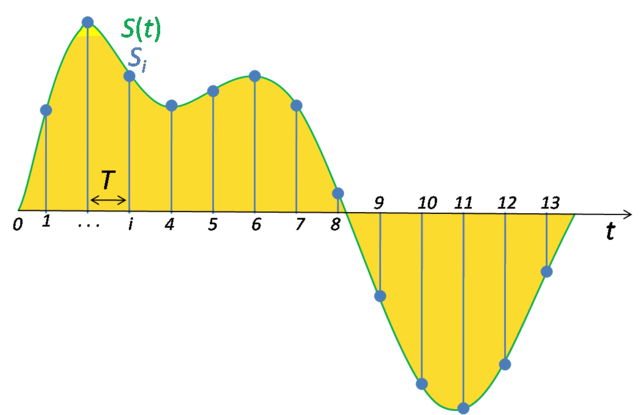
\includegraphics[width=0.6\textwidth]{Signal_Sampling}
%  \caption{Δειγματοληψία ενός αναλογικού σήματος}
%  \label{fig:sampling}
%\end{figure}
%Κατά τη δειγματοληψία ``χάνουμε'' αρκετή από την πληροφορία που περιέχει το αναλογικό σήμα, καθώς οι τιμές που βρίσκονται μεταξύ των διαστημάτων $T_s$ όπου λαμβάνουμε δείγματα δε λαμβάνονται υπόψη. Ακόμη, λόγω της πεπερασμένης ακρίβειας των ψηφιακών συστημάτων για αναπαράσταση αριθμών, η τιμή που έχει το σήμα στρογγυλοποιείται στην πλησιέστερη (είτε μεγαλύτερη είτε μικρότερη) τιμή που μπορεί να αναπαραστήσει το σύστημά μας.
%
%Όπως γίνεται αντιληπτό, σε πολλές των περιπτώσεων η δειγματοληψία μπορεί να έχει καταστροφικές συνέπειες για το αναλογικό σήμα. Ωστόσο, υπό προϋποθέσεις, μπορεί να είναι αντιστρεπτή διαδικασία -- μπορούμε δηλαδή από τα δείγματα που έχουμε λάβει να επιστρέψουμε στην αναλογική μορφή του σήματος. Οι προϋποθέσεις αυτές ορίζονται από το θεώρημα \emph{Shannon-Nyquist} (\ref{thrm:shannon-nyquist}), ως:
%\\
%\begin{theorem}[Shannon-Nyquist]
%	\label{thrm:shannon-nyquist}
%	Ένα σήμα με μέγιστη συχνότητα $f_{max}$ μπορεί να ανακτηθεί από τα δείγματά του, αν αυτά ληφθούν με συχνότητα $f_s>2f_{max}$, ή αλλιώς με περίοδο $T_s<\frac{1}{2f_{max}}$. \cite{proakis_sampling}
%\end{theorem}